\newcommand*{\keyset}{\texttt{keySet}\xspace}
%-----------------------------------------------------------
\subsection{Algorithm $\cctree$: Coreset Tree with  Caching}
\label{sec:cctree}
%-----------------------------------------------------------
The $\cctree$ algorithm uses the idea of ``coreset caching'' to speed up
query processing by reusing coresets that were constructed during prior
queries. In this way, it can avoid merging a large number of coresets at query
time. When compared with $\cstree$, the $\cctree$ algorithm 
is with the same update process ($\ctupdate$), but apply caching
coreset during the query.

%--------------------
\begin{figure*}[tb]
  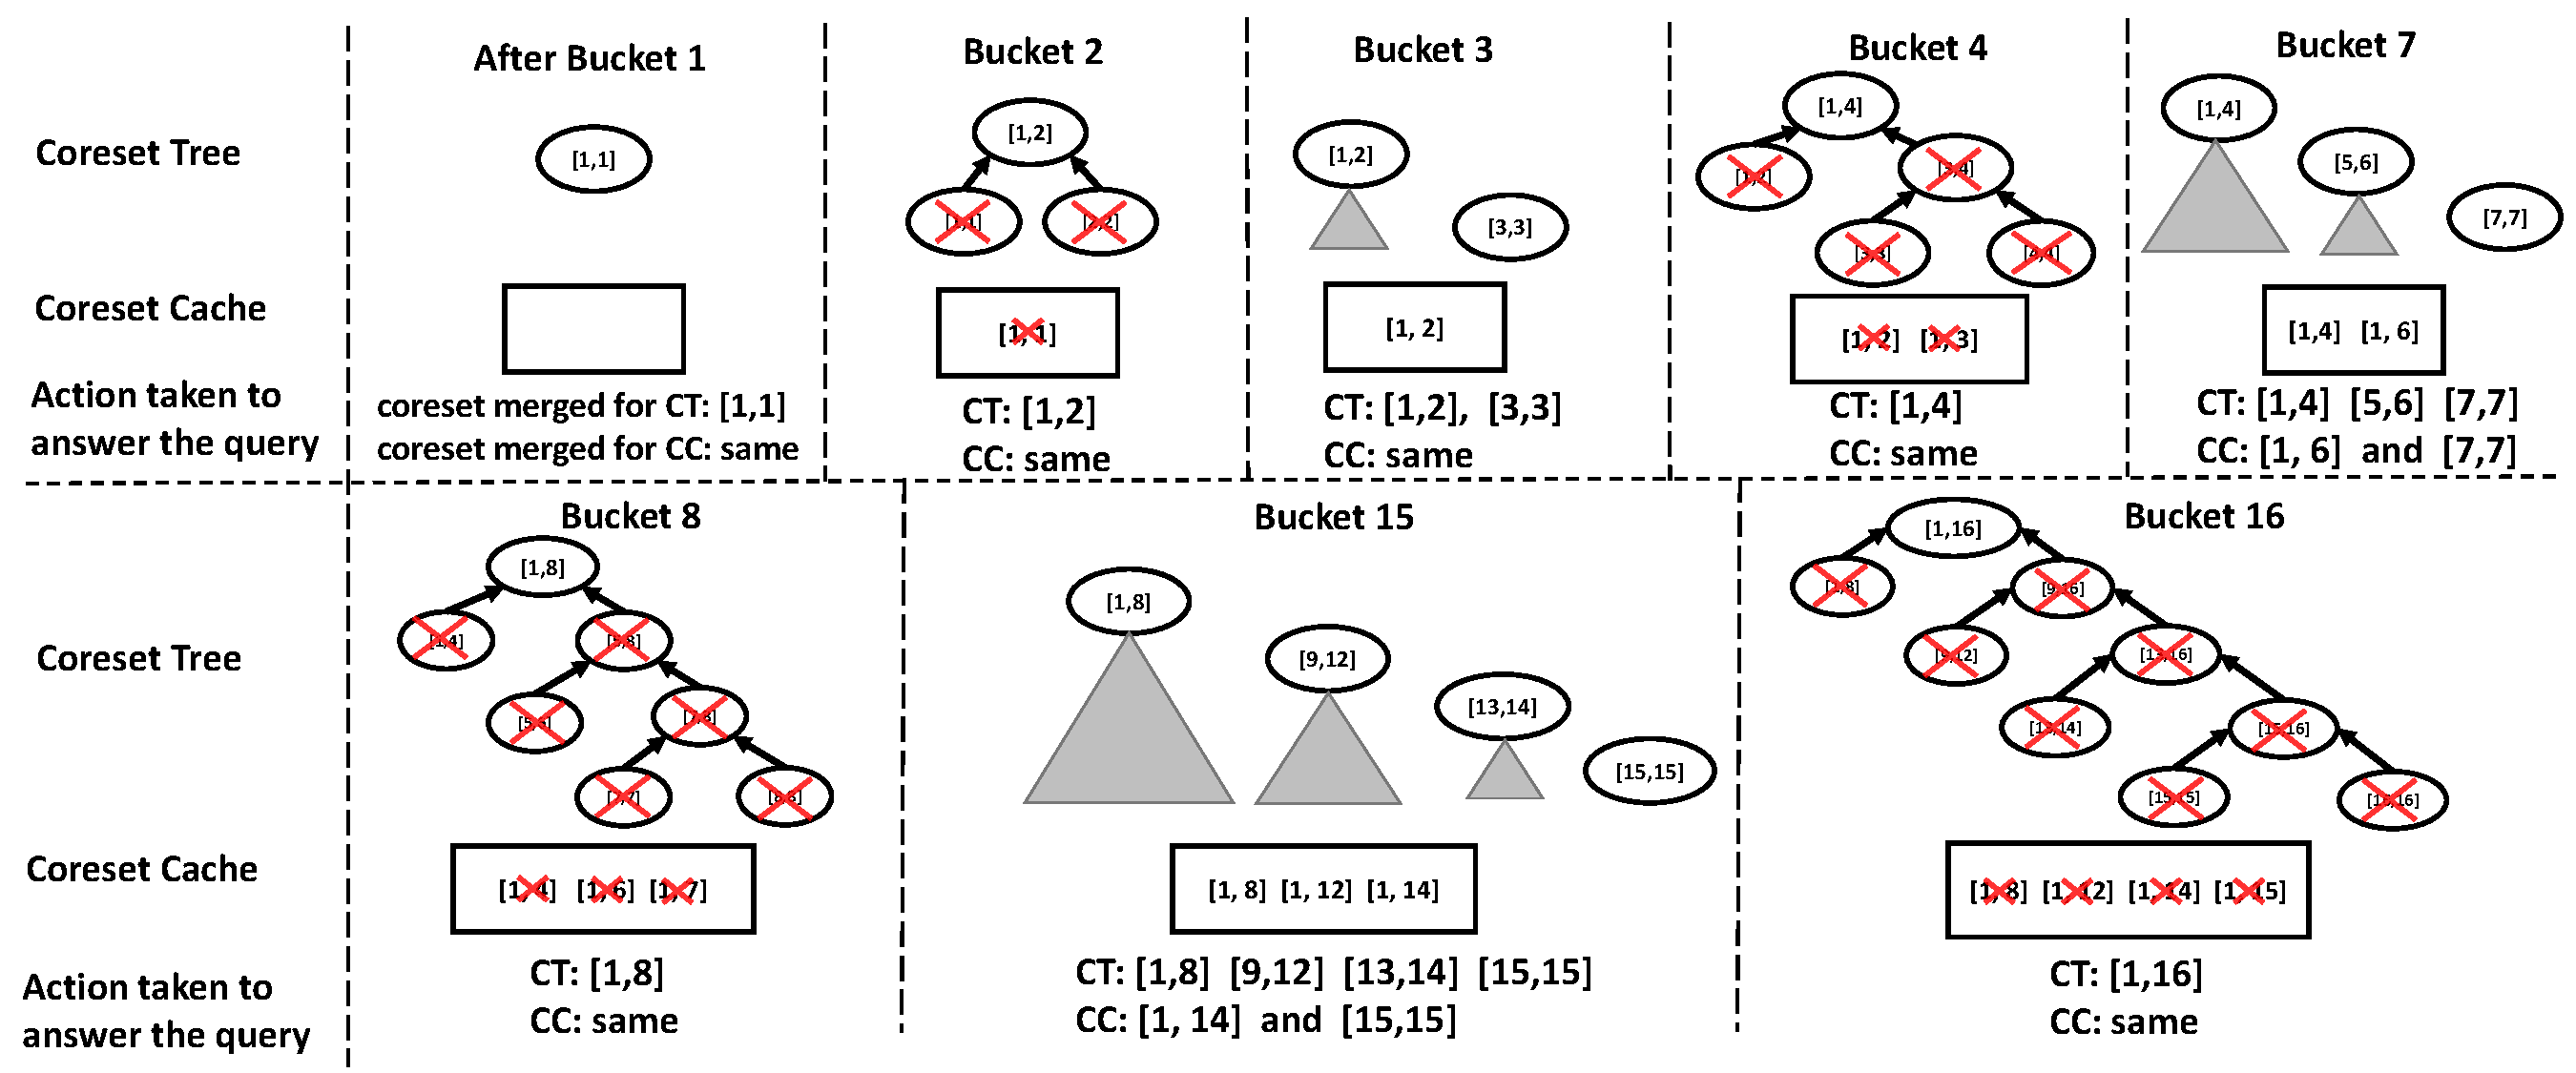
\includegraphics[width=0.98\textwidth]{figs/algo-cc.pdf}
  \caption{Illustration of Algorithm \cc, showing the states of coreset tree and cache after batch $1$, $2$, $3$, $4$, $7$, $8$, $15$ and $16$. The notation $[l,r]$ denotes a coreset of all points in buckets $l$ to $r$, both endpoints inclusive. The coreset tree consists of a set of coresets, each of which is a base bucket or has been formed by merging multiple coresets. Whenever a coreset is merged into a another coreset (in the tree) or discarded (in the cache), the coreset is marked with an ``X''. We suppose that a clustering query arrives after seeing each batch, and describe the actions taken to answer this query (1)~if only \ct was used, or (2)~if \cc was used along with \ct.}
\label{fig:algo-cc}
\end{figure*}
%--------------------

In addition to the coreset tree $\cstree$, the $\cctree$ algorithm
also has an additional \emph{coreset cache} denoted by $\cache$, that stores a
subset of coresets that were previously computed. When a new query has
to be answered, $\cctree$ avoids the cost of merging coresets from
multiple levels in the coreset tree. Instead, it reuses previously
cached coresets and retrieves a small number of additional coresets
which are the same level of the coreset tree, thus leading to less 
computation at query time.

However, the level of the resulting coreset increases linearly with
the number of merges a coreset is involved in. For instance, suppose 
we recursively merge the current coreset with the next arriving base bucket
of coreset to get a new coreset, and so on, for $N$ batches. The resulting 
coreset will have a level of $\Theta(N)$, which can lead to a poor clustering
accuracy. Additional care is needed to ensure that the level of a coreset
is controlled while caching is used.

\noindent\textbf{Details:} Each cached coreset is a summary of base
buckets $1$ through some number $u$. We call this number $u$ as the
\emph{right endpoint} of the coreset and use it as the key/index into
the cache. We call the interval $[1,u]$ as the ``span'' of the
bucket. To explain which coresets can be reused by the algorithm, 
we introduce the following definitions.

%---------------------------------------------
For integers $n > 0$ and $r > 0$, consider the unique decomposition of $n$
according to powers of $r$ as $n = \sum_{i=0}^j \beta_i r^{\alpha_i}$, where
$0 \leq \alpha_0 < \alpha_1 \ldots < \alpha_j$ and $0 < \beta_i < r$ for each
$i$. The $\beta_i$s can be viewed as the non-zero digits in the representation
of $n$ as a number in base $r$. Let $\minor(n,r) = \beta_0 r^{\alpha_0}$, the
smallest term in the decomposition, and $\major(n,r) = n - \minor(n,r)$. Note
that when $n$ is in the form of single term $\beta r^{\alpha}$ 
where $0 < \beta < r$ and $\alpha \geq 0$, $\major(n) = 0$.

For $\kappa =1 \ldots j$, let $n_\kappa = \sum_{i=\kappa}^{j} \beta_i r^{\alpha_i}$. 
$n_\kappa$ can be viewed as the number obtained by dropping the $\kappa$ smallest 
non-zero digits in the representation of $n$ as a number in base $r$. 
The set $\prefixsum(n, r)$ is defined as $\{n_{\kappa} \mid \kappa = 1 \ldots j \}$. 
When $n$ is of the form $\beta r^{\alpha}$ where $0 < \beta < r$, $\prefixsum(n, r)=\emptyset$. 
%---------------------------------------------

For instance, suppose $n=47$ and $r=3$. Since $47 = 1\cdot 3^3 + 2 \cdot 3^2 + 2 \cdot 3^0$, 
we have $\minor(47,3) = 2, \major(47,3) = 45$, and $\prefixsum(47,3) = \{27, 45\}$.

\cc caches every coreset whose right endpoint is in $\prefixsum(N,r)$.
When a query arrives when $N$ buckets received, the task is to compute a coreset
whose span is $[1,N]$. \cc partitions $[1,N]$ as $[1,N_1] \cup [N_1+1,N]$ 
where $N_1 = \major(N,r)$. 
Out of these two intervals, suppose the query comes after every new base bucket received, 
this guarantees that $[1,N_1]$ should be available in the cache. 
$[N_1+1,N]$ is retrieved from the coreset tree, through the union of no more than $(r-1)$ coresets. 
This needs a merge of no more than $r$ coresets. This is in contrast with \ct, 
which may need to merge as many as $(r-1)$ coresets at each level of the tree, 
resulting in a merge of up to $(r-1) \cdot \frac{\log N}{\log r}$ coresets for all levels at query time.

The algorithm for maintaining the cache and answering clustering queries 
is shown in Algorithm~\ref{algo:cctree-functions}. 
The caching process works along with the query process ($\cccoreset$), in a way that
making our algorithm be flexible with the queries by users. When the queries are frequent, 
our algorithm utilizes the cache to provide a faster query speed and a guarantee on the accuracy of 
clustering result. Otherwise in case of the queries are infrequent, we will show that the time complexity 
of updating the cache is at the same level of the query process without caching (algorithm \ct). 
This caching design helps the clustering system to adapt in the faces of both burst queries and occasional queries. 
Figure~\ref{fig:algo-cc} shows an example of how the \cc algorithms updates the cache and answers queries
using cached coresets.

Note that to keep the size of the cache small, as new base buckets arrive,
\ccupdate{} will ensure that ``stale'' or unnecessary coresets are removed. 
The following fact relates to what the cache should store.

%-------------------
\begin{algorithm}
  \caption{Coreset Tree with Caching}
  \label{algo:cctree-functions}
  \label{algo:cctree-init}
  \label{algo:cctree-update}
  \label{algo:cctree-coreset}
\fnDef{$\ccinit(r, k, \eps)$}{
  % Remember the parameters $r$, $k$, and $\eps$.\;
  \tcp{The coreset tree}
  $Q \gets \ctinit{}(r, k, \eps)$ \;
  $\cache \gets \emptyset$
}
\fnDef{$\ccupdate(b,N)$}{
\tcp{$b$ is a new bucket and $N$ is the number of buckets received so far.}
  % Remember $N$\;
  $Q.\ctupdate(b, N)$\;
}
\fnDef{$\cccoreset()$}{
\tcp{Return a coreset of points in buckets $1$ till $N$}
	\uIf{$N$ exists in \cache}
	{
		\Return coreset for buckets $[1, N]$ from the \cache \;
	}
   	$N_1 \gets \major(N,r)$ and $N_2 \gets \minor(N,r)$\;
	Let $N_2=\beta r^{\alpha}$ where $\alpha$ and $\beta < r$ are positive integers\;
	\tcp{coreset for buckets spanning $[1, N_1]$ is not in the \cache}
	\eIf{$N_1$ does not exist in \cache}
	{$U \gets \ctcoreset()$ \;}
	{
		\tcp{$A$ is the coreset for buckets $N_1+1, N_1+2, \ldots, (N_1+N_2)=N$ and is retrieved from the coreset tree}   
   		$a \gets \cup_{B \in Q_\alpha} B$\;
   		\tcp{$b$ is the coreset for buckets spanning $[1, N_1]$, retrieved from the cache} 
   		$b \gets \cache.\lookup(N_1)$ \;
   		$U \gets a \cup b$ \;
   		
	}	
   	\tcp{Store coreset into \cache}
   	%\If{$r$ divides $N$}
   	%{
   		$C \gets \coreset(k, \epsilon, U)$\; 
    	Add coreset $C$ to $\cache$ using key $N$\; 
    	Remove each bucket from $\cache$ whose key does not appear in $\prefixsum(N) \cup \{N\}$  \;
   	%}   
   	\Return {$C$} 
}
\end{algorithm}
%------------------

\begin{fact}
  \label{fact:prefixextension}
  Let $r \geq 2$. For each $N \in \Z^+$,
  $\prefixsum(N+1, r) \subseteq \prefixsum(N,r) \cup \{ N \}$.
\end{fact}
%--------------------------------

Since $\major(N,r) \in \prefixsum(N,r)$ for each $N$, 
if the query comes after each new base bucket received,
we can always retrieve the bucket with span $[1,\major(N,r)]$ from $\cache$.

% -----------------
\begin{lemma}
\label{lemma:cache correctness}
Suppose query comes after receiving each new base bucket. 
Immediately before base bucket $N$ arrives, each $y \in \prefixsum(N,r)$ appears in the key set of \cache.
\end{lemma}
%---------------
\begin{proof}
Proof is by induction on $N$. 
The base case $N=1$ is trivially true, since $\prefixsum(1,r)$ is empty set. 
For the inductive step, assume that before bucket $N$ arrives, 
each $y \in \prefixsum(N, r)$ appears in $\cache$. 
During the query after receiving bucket $N$, 
we store the coreset whose span is $[1, N]$ to the cache.
By Fact~\ref{fact:prefixextension}, we know that
$\prefixsum(N+1, r) \subseteq \prefixsum(N,r) \cup \{N\}$. 
Using this, every bucket with a right endpoint in $\prefixsum(N+1,r)$ 
is present in $\cache$ at the beginning of bucket $(N+1)$ arrives. 
Hence, the inductive step is proved.
\end{proof}
%-----------------

When the queries come less frequent, the cache is less frequently updated as well. 
Then it can not guarantee that the \major is in the cache, that is $N_1$ may not 
exist in the \cache. In this case, the $\cccoreset$ will switch back to the $\ctcoreset$ method in \ct. 
We analyze the time complexity of algorithm $\cc$ under the assumption that we can always use cache 
to accelerate the current query. In practice, we run experiments to show the result of 
algorithm performance when less frequent queries.

%-----------------
\begin{lemma}
\label{lemma:cctree-level}
When queried after inserting base bucket $N$, Algorithm~\cccoreset returns a coreset 
whose level in no more than $\left\lceil 2 \log_r N \right\rceil - 1$.
\end{lemma}
%-----------------
\begin{proof}
Let $\chi(N)$ denote the number of non-zero digits in the representation of $N$ as a number in base $r$. 
We show that the level of the coreset returned by Algorithm~\cccoreset is no more than 
$\left\lceil \log_r N \right\rceil + \chi(N)-1$. 
Since $\chi(N) \le \left\lceil \log_r N \right\rceil$, the lemma follows.

The proof is by induction on $\chi(N)$. If $\chi(N)=1$, then $\major(N,r)=0$,
and the coreset is retrieved directly from the coreset tree $Q$. 
By Fact~\ref{fact:cstree-fact}, each coreset in $Q$ is at a level 
no more than $\lceil \log_r N \rceil$, and the base case follows. 
Suppose the claim was true for all $N$ such that $\chi(N) = t$. Consider $N$ such that
$\chi(N)=(t+1)$. The algorithm computes $N_1 = \major (N,r)$, and retrieves the
coreset with span $[1,N_1]$ from the cache. Note that $\chi(N_1) = t$. By the
inductive hypothesis, the coreset for span $[1,N_1]$ is at a level
$\left\lceil \log_r N \right\rceil + t - 1$. The coresets for span
$[N_1+1,N]$ are retrieved from the coreset tree; note there are multiple such
coresets, but each of them is at a level no more than
$\left\lceil \log_r N \right\rceil$, using Fact~\ref{fact:cstree-fact}.  
The level of the union coreset for span $[1,N]$ is no more than
$\left\lceil \log_r N \right\rceil + t$, proving the inductive case.
\end{proof}
%-----------------

With the coreset level bounded, we can give the guarantee on the accuracy of clustering centers.
Let the accuracy parameter $\eps=\frac{c \log r}{2\log N}$, where $c < \ln{1.1}$.
%-----------------
\begin{lemma}
\label{lemma:cctree-accuracy}
After observing $N$ buckets from the stream, when using clustering data structure \cc, 
Algorithm~\clusterquery returns a set of $k$ points whose clustering cost 
is within a factor of $O(\log k)$ of the optimal $k$-means clustering cost.
\end{lemma}
%-----------------
\begin{proof}
The proof is similar as Lemma~\ref{lemma:cstree-accuracy}. From Lemma~\ref{lemma:cctree-level}, 
we know that the level of a coreset returned is no more than $\left\lceil 2 \log_r N \right\rceil - 1$. 
Using Lemma~\ref{lemma:cstree-level2}, the returned coreset, say $C$, is an $\eps'$-coreset where 
$\eps' = \left[ \left(1 + \frac{{c}\log r}{2\log N}\right)^{\frac{2\log N}{\log r}} - 1 \right] \le \left[ e^{\left(\frac{{c}\log r}{2\log N}\right) \cdot \frac{2\log N}{\log r}}-1 \right] < 0.1$.
Following an argument similar to that of Lemma~\ref{lemma:cstree-accuracy}, we arrive at the result.
\end{proof}
%----------------------

The following lemma shows the time and space complexity of the \cache. 
We show that the time on updating the \cache is at least at the same level of 
the time of answering a query in Algorithm~$\ct$, and can be better to be in linear
scale of $r$ instead of $\frac{r \log N}{\log r}$.
%-----------------------
\begin{lemma}
\label{lemma:cctree-time}
Algorithm~\ref{algo:cctree-update} processes a stream of points 
using amortized time $O(dm)$ per point, 
using memory of $O\left(dm \cdot \frac{r \log N}{\log r} \right)$. 
The amortized cost of answering a query is $O\left(\frac{kdm}{q} \cdot r \right)$.
\end{lemma}
%-----------------

%-----------------
\begin{proof}
The runtime for Algorithm~\ccupdate~ is same as the Algorithm~\ctupdate. 
The update time for \ccupdate is $O(dm)$ per point.

From Lemma~\ref{lemma:cache correctness}, $N_1$ is always in the \cache. 
Algorithm~\cccoreset combines no more than $r$ buckets, 
out of which there is no more than one bucket from the cache, 
and no more than $(r-1)$ from the coreset tree. 
From Theorem~\ref{theo:coreset-build}, the time to compute coreset 
on $O(mr)$ points is $O(d m^2 r)$, and coreset size $m$ is $O(k)$.
The time to compute coreset $C$ is $O(kdmr)$.   
To compute the $k$ centers from $U$, 
it is necessary to run $\kmpp$ on $O(mr)$ points using time $O(kdmr)$. 
The amortized query time per point is $O\left( \frac{kdmr}{q} \right)$.

\remove {
In the worst case, when the major part is always not in the cache. 
Comparing to Algorithm~\ct, the additional time cost is updating the cache. 
The number of points in set $U$ is at most $(m \cdot \frac{r \log N}{\log r})$, 
computation time is $O(d m^2 r \cdot \log_r N)$. 
As the size of coreset is $O(k)$, 
the addition time for constructing coreset is $O(kdm \cdot \frac{r \log N}{\log r})$ 
at the same level of the query time by \ct.
}

The coreset tree $Q$ uses space $O\left( dm \cdot \frac{r \log N}{\log r} \right)$. 
After processing bucket $N$, $\cache$ only stores those buckets that are 
corresponding to $\prefixsum(N,r) \cup \{ N \}$. 
The number of such buckets possible is $O(\log_r N )$, 
so the space cost of $\cache$ is $O(dm \cdot \frac{\log N}{\log r})$. 
The space complexity follows.
\end{proof}
%-----------------

